\documentclass[12pt,a4paper]{report}

\usepackage[a4paper,hscale=0.65,vscale=0.71]{geometry}

\usepackage{isabelle,isabellesym}

\usepackage{charter}

\usepackage{tikz}
\usetikzlibrary{shadows}

\usepackage{listings}

\usepackage{alltt}

\usepackage{railsetup}

% this should be the last package used
\usepackage{pdfsetup}

% urls in roman style, theory text in math-similar italics
\urlstyle{rm}
\isabellestyle{tt}

\renewcommand{\isastyleminor}{\tt}

\lstdefinelanguage{SPARK}[95]{Ada} {
   morecomment=*[l]{--\#},
   morekeywords=
   {
     inherit, own, initializes, hide, global, main_program,
     derives, from, pre, post, return, assert, check
   }
}

\lstset{ %
language=SPARK,
basicstyle=\small\ttfamily,
keywordstyle=\rmfamily\bfseries,
columns=flexible,
showstringspaces=false
}

\newcommand{\mod}{\mathbin{\hbox{\textbf{mod}}}}

\newcommand{\SPARK}{\textsc{Spark}}

\newcommand{\secref}[1]{\S \ref{#1}}
\newcommand{\figref}[1]{Fig.\ \ref{#1}}

\renewcommand{\topfraction}{.99}
\renewcommand{\bottomfraction}{.99}
\setcounter{topnumber}{9}
\setcounter{bottomnumber}{9}
\setcounter{totalnumber}{20}


\begin{document}

\title{The HOL-\SPARK{} Program Verification Environment}
\author{\emph{Stefan Berghofer} \\ \emph{secunet Security Networks AG}}
\maketitle

\tableofcontents

% sane default for proof documents
\parindent 0pt\parskip 0.5ex

\chapter{Introduction}
\label{sec:intro}

This document describes a link between Isabelle/HOL and the \SPARK{}/Ada tool
suite for the verification of high-integrity software.
Using this link, verification problems can be tackled that are beyond reach
of the proof tools currently available for \SPARK{}. A number of examples
can be found in the directory \texttt{HOL/SPARK/Examples} in the Isabelle
distribution. An open-source version of the \SPARK{} tool suite is available
free of charge from \hbox{\href{http://libre.adacore.com}{libre.adacore.com}}.

In the remainder of \secref{sec:intro},
we give an introduction to \SPARK{} and the HOL-\SPARK{} link. The verification
of an example program is described in \secref{sec:example-verification}. In
\secref{sec:vc-principles}, we explain the principles underlying the generation
of verification conditions for \SPARK{} programs. Finally, \secref{sec:spark-reference}
describes the commands provided by the HOL-\SPARK{} link, as well as the encoding
of \SPARK{} types in HOL.

\section{\SPARK{}}

\SPARK{} \cite{Barnes} is a subset of the Ada language that has been designed to
allow verification of high-integrity software. It is missing certain features of
Ada that can make programs difficult to verify, such as \emph{access types},
\emph{dynamic data structures}, and \emph{recursion}. \SPARK{} allows to prove
absence of \emph{runtime exceptions}, as well as \emph{partial correctness}
using pre- and postconditions. Loops can be annotated with \emph{invariants},
and each procedure must have a \emph{dataflow annotation}, specifying the
dependencies of the output parameters on the input parameters of the procedure.
Since \SPARK{} annotations are just written as comments, \SPARK{} programs can be
compiled by an ordinary Ada compiler such as GNAT. \SPARK{} comes with a number
of tools, notably the \emph{Examiner} that, given a \SPARK{} program as an input,
performs a \emph{dataflow analysis} and generates \emph{verification conditions}
(VCs) that must be proved in order for the program to be exception-free and partially
correct. The VCs generated by the Examiner are formulae expressed in
a language called FDL, which is first-order logic extended with
arithmetic operators, arrays, records, and enumeration types. For example,
the FDL expression
\begin{alltt}
  for_all(i: integer, ((i >= min) and (i <= max)) ->
    (element(a, [i]) = 0))
\end{alltt}
states that all elements of the array \texttt{a} with indices greater or equal to
\texttt{min} and smaller or equal to \texttt{max} are $0$.
VCs are processed by another \SPARK{} tool called the
\emph{Simplifier} that either completely solves VCs or transforms them
into simpler, equivalent conditions. The latter VCs
can then be processed using another tool called
the \emph{Proof Checker}. While the Simplifier tries to prove VCs in a completely
automatic way, the Proof Checker requires user interaction, which enables it to
prove formulae that are beyond the scope of the Simplifier. The steps
that are required to manually prove a VC are recorded in a log file by the Proof
Checker. Finally, this log file, together with the output of the other \SPARK{} tools
mentioned above, is read by a tool called POGS (\textbf{P}roof \textbf{O}bli\textbf{G}ation
\textbf{S}ummariser) that produces a table mentioning for each VC the method by which
it has been proved.
In order to overcome the limitations of FDL and to express complex specifications,
\SPARK{} allows the user to declare so-called
\emph{proof functions}. The desired properties of such functions are described
by postulating a set of rules that can be used by the Simplifier and Proof Checker
\cite[\S 11.7]{Barnes}. An obvious drawback of this approach is that incorrect
rules can easily introduce inconsistencies.

\section{HOL-\SPARK{}}

The HOL-\SPARK{} verification environment, which is built on top of Isabelle's object
logic HOL, is intended as an alternative
to the \SPARK{} Proof Checker, and improves on it in a number of ways.
HOL-\SPARK{} allows Isabelle to directly parse files generated
by the Examiner and Simplifier, and provides a special proof command to conduct
proofs of VCs, which can make use of the full power of Isabelle's rich
collection of proof methods.
Proofs can be conducted using Isabelle's graphical user interface, which makes
it easy to navigate through larger proof scripts. Moreover, proof functions
can be introduced in a \emph{definitional} way, for example by using Isabelle's
package for recursive functions, rather than by just stating their properties as axioms,
which avoids introducing inconsistencies.

\begin{figure}
\begin{center}
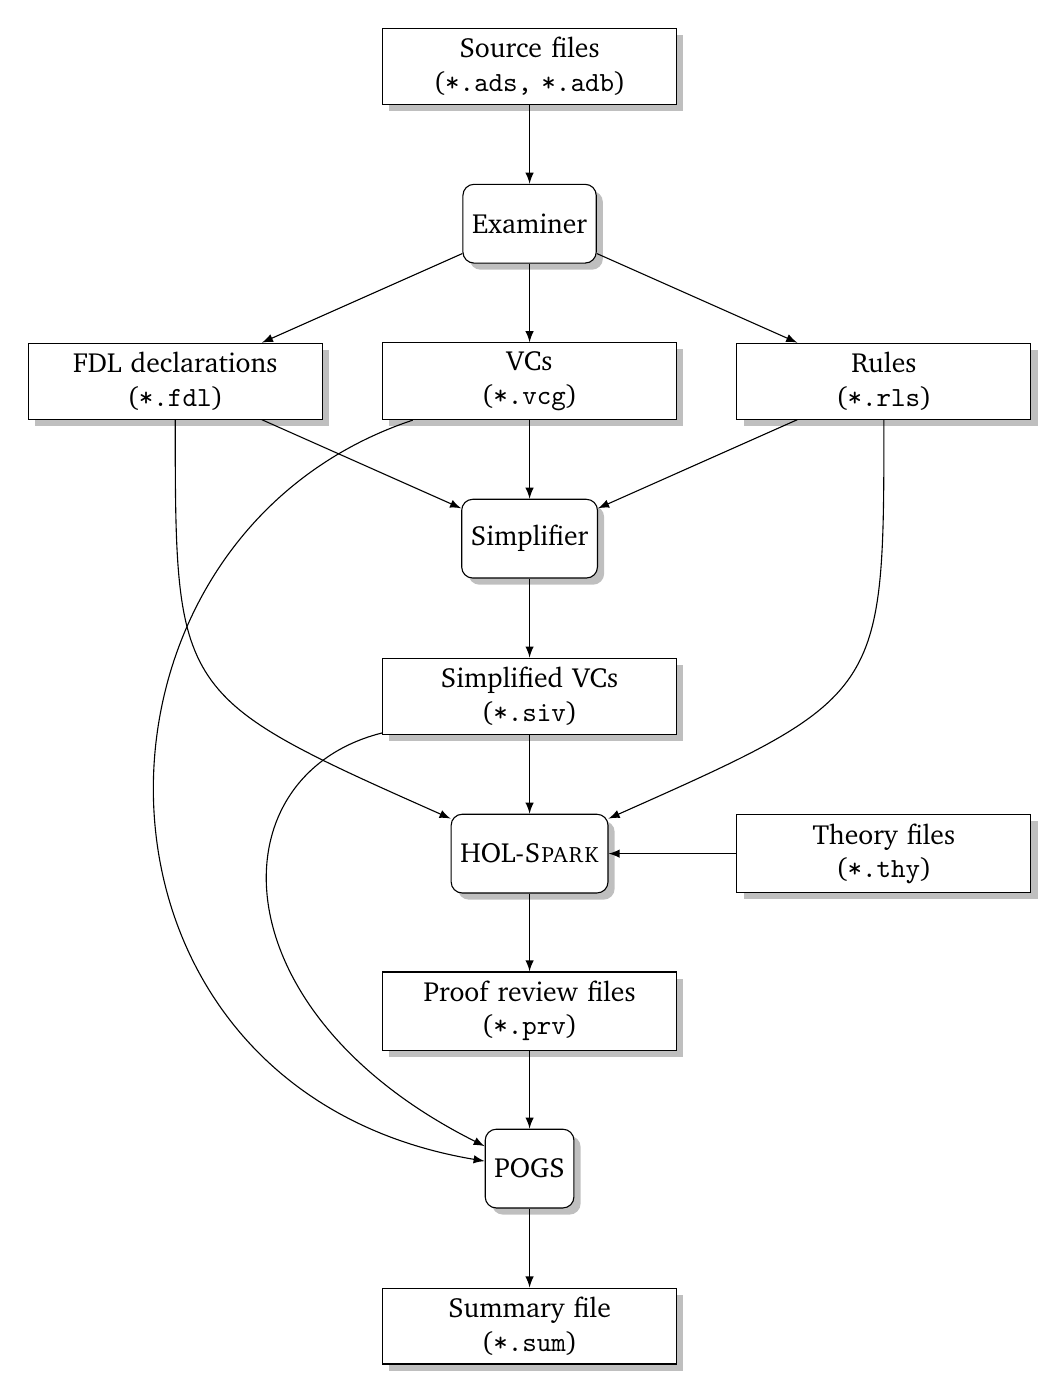
\begin{tikzpicture}
\tikzstyle{box}=[draw, drop shadow, fill=white, text width=3.5cm, text centered]
\tikzstyle{rbox}=[draw, drop shadow, fill=white, rounded corners, minimum height=1cm]

\node[box] (src) at (5,0) {Source files (\texttt{*.ads, *.adb})};
\node[rbox] (exa) at (5,-2) {Examiner};
\node[box] (fdl) at (0.5,-4) {FDL declarations \\ (\texttt{*.fdl})};
\node[box] (vcs) at (5,-4) {VCs \\ (\texttt{*.vcg})};
\node[box] (rls) at (9.5,-4) {Rules \\ (\texttt{*.rls})};
\node[rbox] (simp) at (5,-6) {Simplifier};
\node[box] (siv) at (5,-8) {Simplified VCs \\ (\texttt{*.siv})};
\node[rbox] (isa) at (5,-10) {HOL-\SPARK{}};
\node[box] (thy) at (9.5,-10) {Theory files \\ (\texttt{*.thy})};
\node[box] (prv) at (5,-12) {Proof review files \\ (\texttt{*.prv})};
\node[rbox] (pogs) at (5,-14) {POGS};
\node[box] (sum) at (5,-16) {Summary file \\ (\texttt{*.sum})};

\draw[-latex] (src) -- (exa);
\draw[-latex] (exa) -- (fdl);
\draw[-latex] (exa) -- (vcs);
\draw[-latex] (exa) -- (rls);
\draw[-latex] (fdl) -- (simp);
\draw[-latex] (vcs) -- (simp);
\draw[-latex] (rls) -- (simp);
\draw[-latex] (simp) -- (siv);
\draw[-latex] (fdl) .. controls (0.5,-8) .. (isa);
\draw[-latex] (siv) -- (isa);
\draw[-latex] (rls) .. controls (9.5,-8) .. (isa);
\draw[-latex] (thy) -- (isa);
\draw[-latex] (isa) -- (prv);
\draw[-latex] (vcs) .. controls (-1,-6) and (-1,-13) .. (pogs);
\draw[-latex] (siv) .. controls (1,-9) and (1,-12) .. (pogs);
\draw[-latex] (prv) -- (pogs);
\draw[-latex] (pogs) -- (sum);
\end{tikzpicture}
\end{center}
\caption{\SPARK{} program verification tool chain}
\label{fig:spark-toolchain}
\end{figure}
Figure \ref{fig:spark-toolchain} shows the integration of HOL-\SPARK{} into the
tool chain for the verification of \SPARK{} programs. HOL-\SPARK{} processes declarations
(\texttt{*.fdl}) and rules (\texttt{*.rls}) produced by the Examiner, as well as
simplified VCs (\texttt{*.siv}) produced by the \SPARK{} Simplifier. Alternatively,
the original unsimplified VCs (\texttt{*.vcg}) produced by the Examiner can be
used as well. Processing of the \SPARK{} files is triggered by an Isabelle
theory file (\texttt{*.thy}), which also contains the proofs for the VCs contained
in the \texttt{*.siv} or \texttt{*.vcg} files. Once that all verification conditions
have been successfully proved, Isabelle generates a proof review file (\texttt{*.prv})
notifying the POGS tool of the VCs that have been discharged.

\input{Example_Verification}
\input{VC_Principles}
\input{Reference}

% optional bibliography
\bibliographystyle{abbrv}
\bibliography{root}

\end{document}

%%% Local Variables:
%%% mode: latex
%%% TeX-master: t
%%% End:
